\chapter{初段ミューオントリガーシステム}\label{chapter3}
ATLAS実験における初段ミューオントリガーは、RPCを用いるバレル部とTGCを用いるエンドキャップ部に分かれている。
本章では、Run-3におけるエンドキャプ部の初段ミューオントリガーシステムについて述べる。

\section{エンドキャプ部初段ミューオントリガー}
%図~\ref{fig:muon}に示すように
エンドキャプ部の初段ミューオントリガーはさらに2つの領域に分けられ、$1.05 < |\eta| < 1.9$をエンドキャップ領域、$1.9 < |\eta| < 2.4$をフォワード領域と呼ぶ。
%\begin{figure}[tb]
%  \centering
%  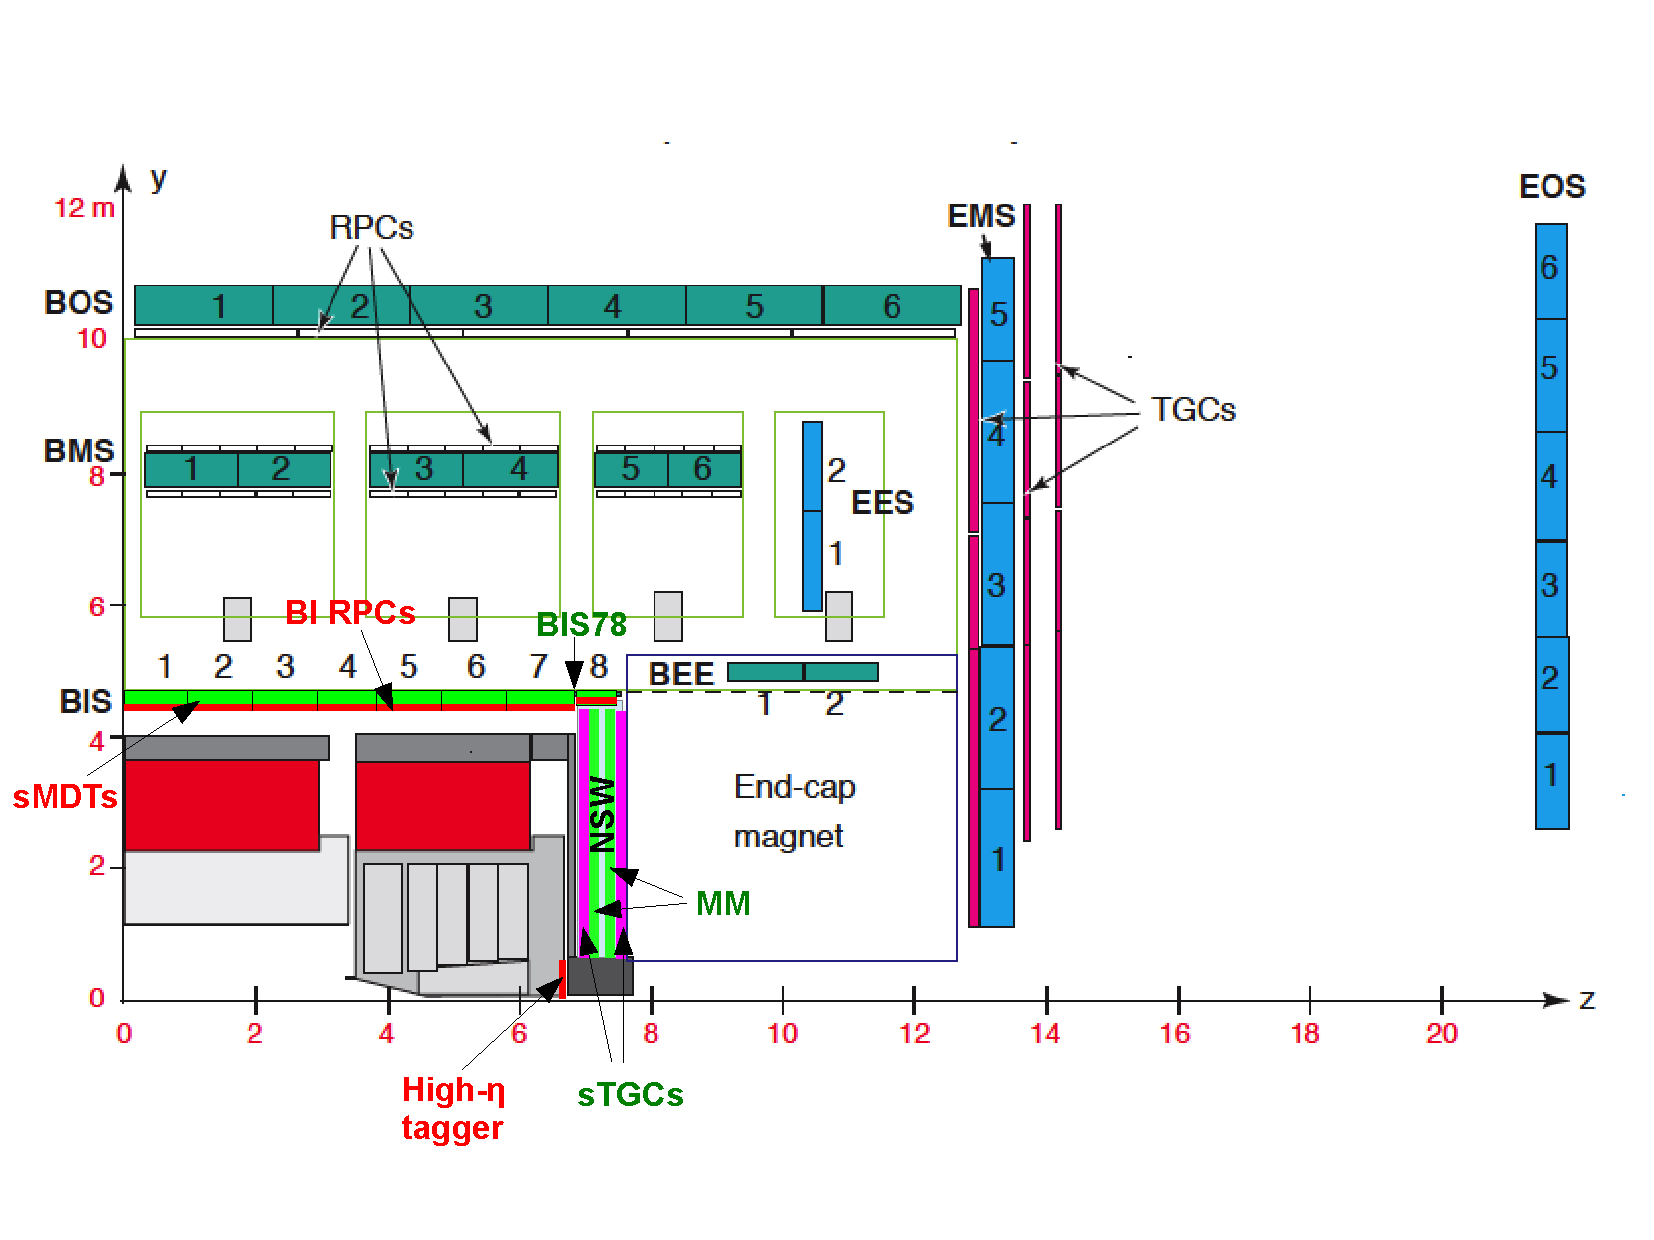
\includegraphics[clip, width=14cm]{fig/2/ch01_fig_03a.pdf}
%  \caption{初段ミューオントリガーに用いる検出器の設置位置\cite{article:phase2}。バレル部のトリガー判定に用いるRPCと、エンドキャップ部のトリガー判定に用いるTGCがATLAS検出器の最外層に設置されている。}
%  \label{fig:muon}
%\end{figure}

\subsection{トリガーアルゴリズムの概要}\label{section:CW}

\subsubsection{ミューオンの横方向運動量の判定}
エンドキャップ部の初段ミューオントリガーで用いられるトリガー判定の概要を図~\ref{fig:trigger-scheme}に示す。
衝突点で生成されたミューオンはトロイド磁石の磁場領域より内側にある検出器を通過した後、トロイド磁場領域を通りTGCに到達する。トロイド磁石による磁場は$\phi$方向にかかっているため、ミューオンの飛跡はトロイド磁場中で$\eta$方向に曲げられる。さらに、衝突点付近のソレノイド磁石で生じる$z$方向の磁場成分と、トロイド磁石付近で生じた$R$方向の磁場成分によって、ミューオンの飛跡は$\phi$方向にも曲げられる。ミューオンの飛跡の曲がり具合は横方向運動量$p_{\rm{T}}$の大きさによって変化するため、測定した飛跡情報からミューオンの$p_{\rm{T}}$を算出することができ、トリガー判定に使用することができる。

トロイド磁場によって曲げられたミューオンは、TGC-BWのM1, M2, M3を通過し、それぞれのヒット情報から飛跡を再構成される。この時、衝突点とM3のヒット位置を結んだ直線をミューオンが無限運動量で通過したと仮定した場合の飛跡として扱う。この無限運動量を持つミューオンの飛跡と磁場によって曲げられた実際の飛跡を比較し、M1におけるヒット位置のR方向と$\phi$方向のずれ(d$R$, d$\phi$)を計算する。このd$R$とd$\phi$の値が大きいミューオンは、磁場中で大きく曲げられたことを意味しているため小さい$p_{\rm{T}}$として判定される。逆にd$R$とd$\phi$の値がが小さいほど、磁場中ではあまり曲がらないミューオンの飛跡であるため大きな$p_{\rm{T}}$として判定される。
初段ミューオントリガーでは(d$R$, d$\phi$)からトリガー判定に用いる$p_{\rm{T}}$を算出する際に、あらかじめ保持しておいた(d$R$, d$\phi$)と$p_{\rm{T}}$の対応関係を表したLook-Up Table~(LUT)を参照することで、短時間での$p_{\rm{T}}$の算出を実現している。

\begin{figure}[tb]
  \centering
  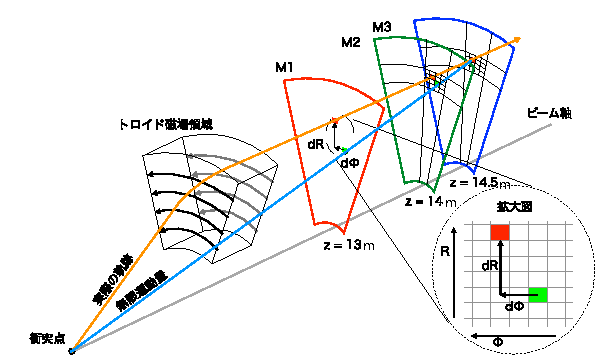
\includegraphics[clip, width=15cm]{fig/3/akatuka_mt_trigger_sceme.pdf}
  \caption{ATLAS検出器エンドキャップ領域におけるトリガースキームの概念図\cite{article:akatsuka-mron}。無限大の運動量を持つミューオンを仮定し、磁場によって曲げられたミューオンとの位置の差(d$R$, d$\phi$)を用いて$p_{\rm{T}}$を計算する。}
  \label{fig:trigger-scheme}
\end{figure}

%LUTとは入力データに対応する出力データを参照するための表のことを指し、初段ミューオントリガーでは、(dR, d$\phi$)を入力として$p_{\rm{T}}$を出力するLUTをFPGAに保存している。

%\subsubsection{Coincidence Window}
$p_{\rm{T}}$を算出する際に参照するLUTはCoincidence Window~(CW)と呼ばれており、図~\ref{fig:CW}のようなCWがFPGA上に保存されている。
図~\ref{fig:CW}のCWが色分けされているように、(d$R$,d$\phi$)によって判定される$p_{\rm{T}}$は異なり、Run-3においては15段階の$p_{\rm{T}}$を判定することができる。この15段階の$p_{\rm{T}}$の閾値は先行研究\cite{article:shiomi-mron}によって定められており、表~\ref{pt_number}に$p_{\rm{T}}$閾値を示す。
このとき、図~\ref{fig:CW}に示すCWのマスの中の数字は表~\ref{pt_number}に示す閾値と対応しており、符号はミューオンの電荷に対応している。
図~\ref{fig:Run3_15_MC5}に2022年Run-3で用いられたCWのトリガー効率を示す。
%Run-3のミューオントリガーで用いられるCWは15段階の$p_{\rm{T}}$を判定することができ、図~\ref{fig:CW}に示すCWの15色がそれぞれ15段階の
%判定できる$p_{\rm{T}}$は、図~\ref{fig:CW}の15色が示すように15段階である。マスの中の数字は表~\ref{pt_number}に示す$p_{\rm{T}}$ numberと対応している。また、各$p_{\rm{T}}$閾値の符号はミューオンの電荷に対応している。図~\ref{fig:CW}の
%エンドキャップ部のトロイド磁場やTGCは理想的には8回対称であるが、磁場の向きやTGCチェンバーの設置位置のズレなどがあるため、CWはTGC-BWのトリガー判定に用いられる単位位置情報ごとに独立に作成されている。

\begin{figure}[tb]
  \centering
  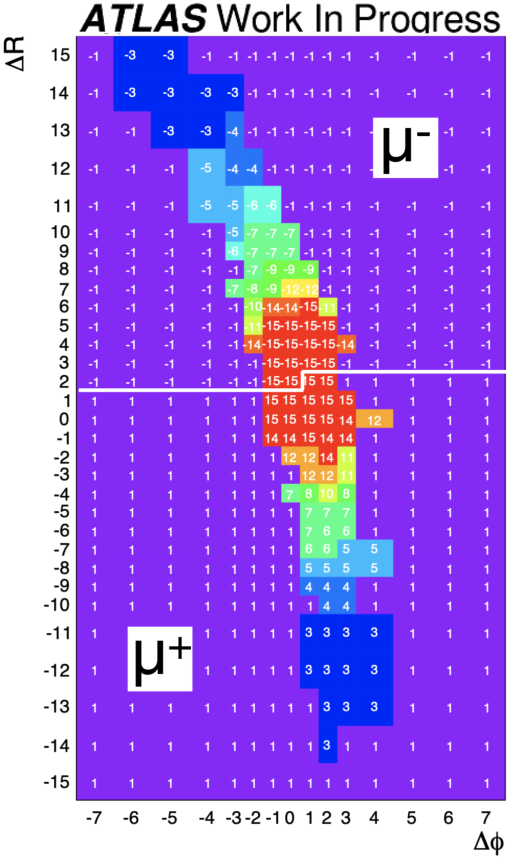
\includegraphics[clip, width=7cm]{fig/3/Run3CW.pdf}
  \caption{Run-3でのTGCにおける3ステーションのCoincidence Windowの例\cite{article:shiomi-mron}。ミューオンのヒットがあった時にそれぞれの検出位置ののCWを参照し、(d$R$, d$φ$)からミューオンの$p_{\rm{T}}$を15段階で見積もる。マスの中の数字は表~\ref{pt_number}に示す閾値と対応しており、符号はミューオンの電荷に対応している。}
  \label{fig:CW}
\end{figure}

\begin{table}[]
    \caption{Run-3初段ミューオントリガーにおける15段階の$p_{\rm{T}}$閾値\cite{article:shiomi-mron}。}
    \label{pt_number}
    \centering
    %\begin{tabular}{|c|c|c|c|c|c|c|c|c|c|c|c|c|c|c|c|c|c|c|c|c|c|c|c|}
    \begin{tabular}{|c|c|c|c|}
        \hline
        閾値番号 & L1 items & 条件\\
        \hline
        1 & L1$\_$MU3 & $p_{\rm{T}} \geq$ 3 GeV \\
        \hline
        2 & L1$\_$MU4 & $p_{\rm{T}} \geq$ 4 GeV \\
        \hline
        3 & L1$\_$MU5 & $p_{\rm{T}} \geq$ 5 GeV \\
        \hline
        4 & L1$\_$MU6 & $p_{\rm{T}} \geq$ 6 GeV \\
        \hline
        5 & L1$\_$MU7 & $p_{\rm{T}} \geq$ 7 GeV \\
        \hline
        6 & L1$\_$MU8 & $p_{\rm{T}} \geq$ 8 GeV \\
        \hline
        7 & L1$\_$MU9 & $p_{\rm{T}} \geq$ 9 GeV \\
        \hline
        8 & L1$\_$MU10 & $p_{\rm{T}} \geq$ 10 GeV \\
        \hline
        9 & L1$\_$MU11 & $p_{\rm{T}} \geq$ 11 GeV \\
        \hline
        10 & L1$\_$MU12 & $p_{\rm{T}} \geq$ 12 GeV \\
        \hline
        11 & L1$\_$MU13 & $p_{\rm{T}} \geq$ 13 GeV \\
        \hline
        12 & L1$\_$MU14 & $p_{\rm{T}} \geq$ 14 GeV \\
        \hline
        13 & L1$\_$MU15 & $p_{\rm{T}} \geq$ 15 GeV \\
        \hline
        14 & L1$\_$MU18 & $p_{\rm{T}} \geq$ 18 GeV \\
        \hline
        15 & L1$\_$MU20 & $p_{\rm{T}} \geq$ 20 GeV \\
        \hline
        %$p_{\rm{T}}$ number & 1 & 2 & 3 & 4 & 5 & 6 & 7 & 8 & 9 & 10 & 11 & 12 & 13 & 14 & 15\\
        %\hline
        %$p_{\rm{T}}$ Threshould[GeV] & 3 & 4 & 5 & 6 & 7 & 8 & 9 & 10 & 11 & 12 & 13 & 14 & 15 & 18 & 20\\
        %$p_{\rm{T}}$ Threshould& 3 & 4 & 5 & 6 & 7 & 8 & 9 & 10 & 11 & 12 & 13 & 14 & 15 & 18 & 20\\
        %\hline
    \end{tabular}
\end{table}

\begin{figure}[tb]
  \centering
  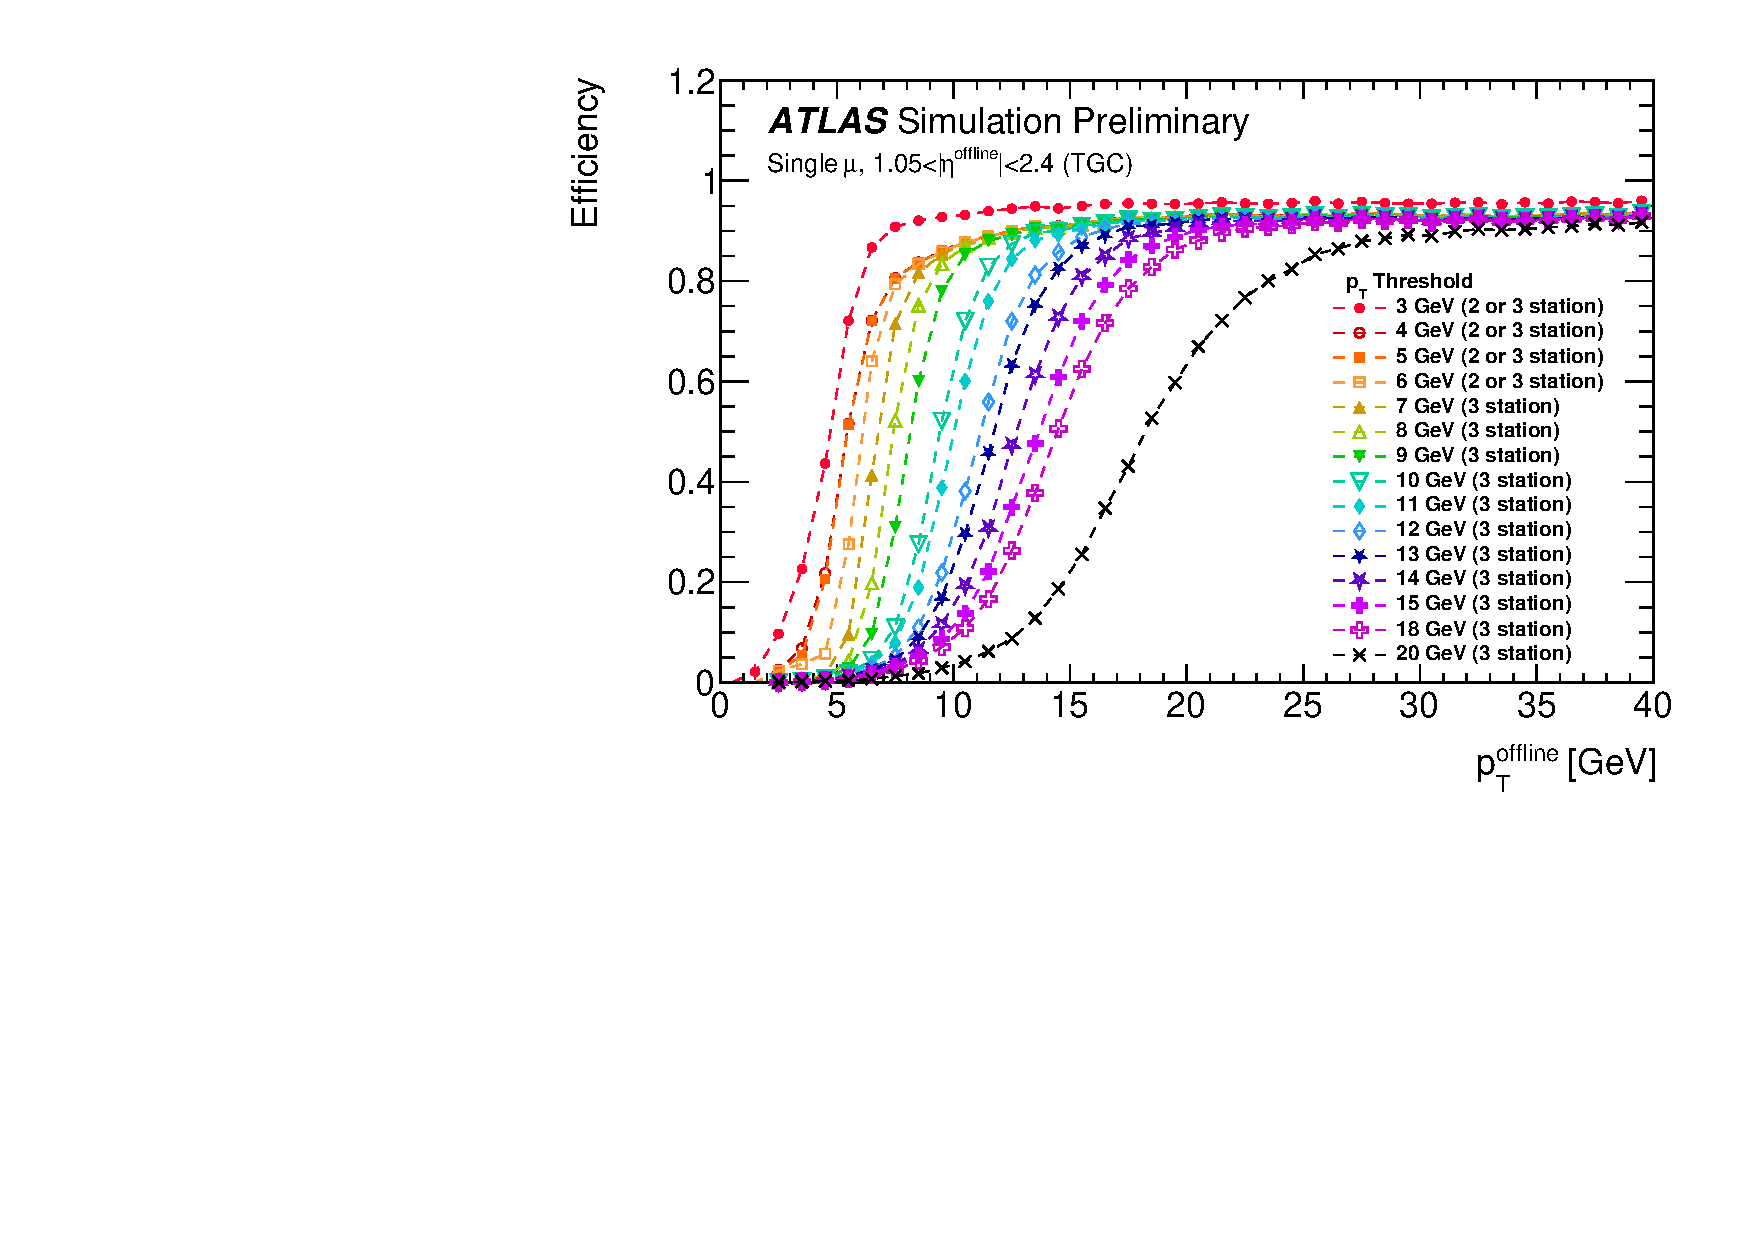
\includegraphics[clip, width=14cm]{fig/3/PLOT-TRIG-2020-01-fig1.pdf}
  \caption{2022年Run-3で使用した15段階閾値のTurn-on curve~\cite{article:shiomi-mron}。シングルミューオンのシミュレーションサンプルに対してのトリガー効率を示している。}
  \label{fig:Run3_15_MC5}
\end{figure}

%また、CWはコインシデンスのタイプによって大きく分けて4種類に分類できる。
%一つ目はM1からM3までの3つのステーション(M1, M2, M3)全てにおいてワイヤーとストリップともにヒットが確認された3ステーションコインシデンス、二つ目がワイヤーは3ステーションにヒットが確認されたが、ストリップに関しては2ステーション(M2, M3)のヒットしか確認できなかった3-2ステーションコインシデンス、三つ目がワイヤーは2ステーションしかヒットが確認されなかったが、ストリップでは3ステーションにヒットが確認された2-3 ステーションコインシデンス、四つ目がワイヤーとストリップともに2ステーションしかヒットが確認できなかった2ステーションコインシデンスである。
%3ステーションコインシデンスフラグはストリップ、ワイヤー共に3ステーションでヒットがあった場合に立つフラグである。
%2ステーションコインシデンスか 3ステーションコインシデンスかでズレを計算する検出器がM2-M3か、M1-M3か変わってくるため、(dR、d$\phi$)の範囲も変わってくる。2ステーションの場合、$−7 \geq dR \geq 7$、$−3 \geq d\phi \geq 3$、3 ステーションの場合、$−15 \geq dR \geq 15$、$−7 \geq d\phi \geq 7$ の範囲で定義される。

\subsubsection{インナーコインシデンス}\label{innnercoin}
エンドキャップ部のミューオントリガーには陽子衝突由来でない荷電粒子により発行されたトリガー~(フェイクトリガー)が存在し、レートを上げる要因になっている。Run-2ではTGCのヒット情報に対してTGC-EI/FIとTileカロリメータの情報を使ったコインシデンス~(インナーコインシデンス) を取ることでフェイクトリガーを大きく削減することができた。しかし、$1.9 < |\eta| < 2.4$ の領域ではインナーコインシデンスをとるためのトリガー用検出器がないためフェイクトリガーが多く残っていた。
Run-3からはNSWとRPC~BIS78の導入により、Run-2より広範囲でインナーコインシデンスをとることが可能になり、フェイクトリガーをより削減できることが期待される。
Tileカロリメータとコインシデンスだけでなく、新たに導入されるNSWやRPC~BIS78をインナーコインシデンスに用いた場合に期待されるトリガー発行数の分布を図\ref{fig:Rate_innercoincidence}に示す。

\begin{figure}[tb]
  \centering
    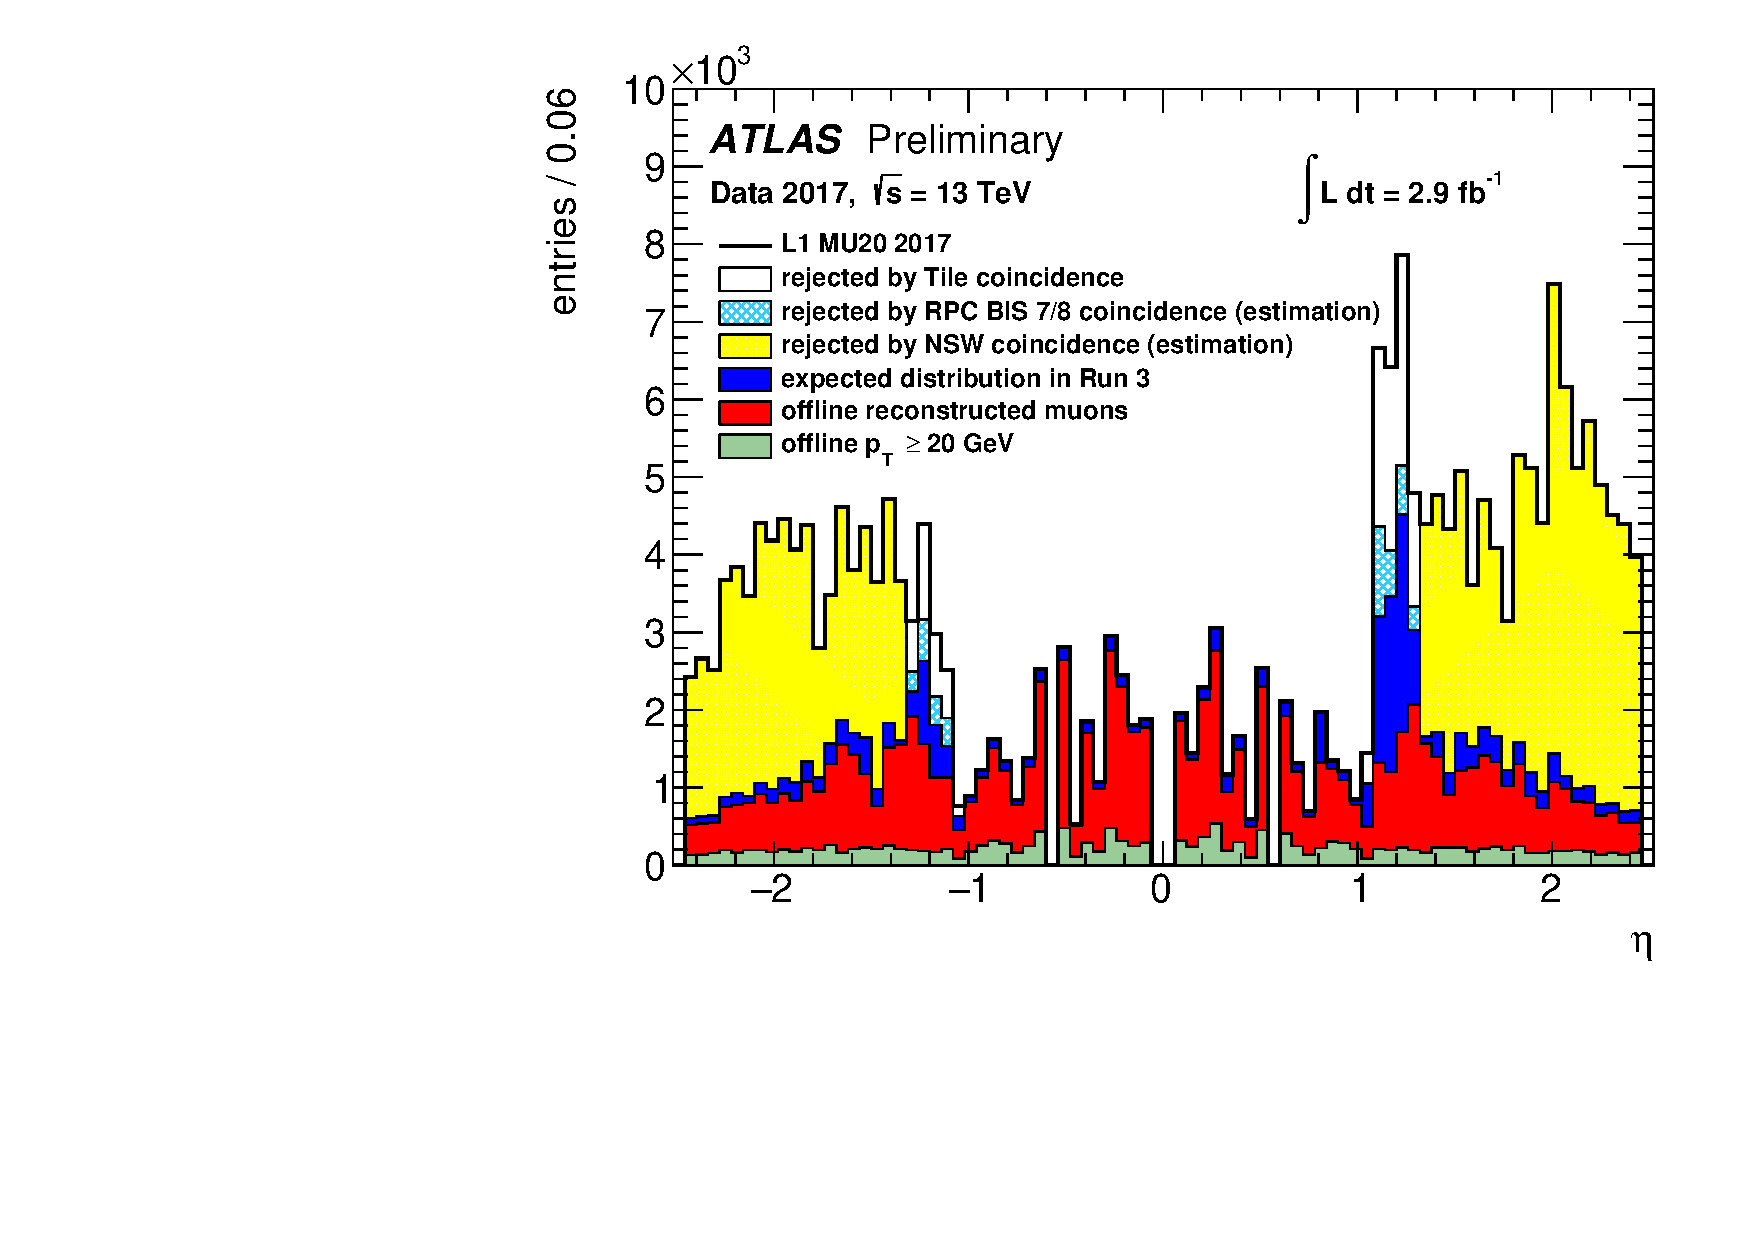
\includegraphics[clip, width=14cm]{fig/3/ATL-COM-DAQ-2018-033-fig2.pdf}
  \caption{Run-3 で期待される $p_{\rm{T}}$閾値が20~GeVにおけるトリガー発行数の$\eta$分布\cite{article:ATLASpublic}。白色、水色、黄色の領域はそれぞれ Tile カロリメータ、RPC BIS78、NSWを用いたインナーコインシデンスを導入した場合に削減できるトリガー発行数を示す。青色の領域は Run-3で期待されるトリガー発行数、赤色の領域は発行されたトリガーのうちオフラインで再構成されるミューオンの数を示す。緑の分布はオフラインで再構成されたミューオンのうち、$p_{\rm{T}}$が20~GeV以上のミューオンの数を示す。}
  \label{fig:Rate_innercoincidence}
\end{figure}

\subsubsection{トリガー判定に用いられる位置情報}
TGC のトリガー判定に用いられる単位の模式図を図~\ref{fig:RoI}に示す。
TGCの検出領域は$\phi$方向にエンドキャプ領域では48個、フォワード領域では24個に分割しており、トリガー回路的に独立していて "トリガーセクター" と呼ばれる。このトリガーセクターはさらに小さな領域であるRegion of Interest~(RoI)に分割され、エンドキャップ領域のトリガーセクターは$\eta$方向に37分割、$\phi$方向に4分割されるため148個のRoIで構成されている。フォワード領域のトリガーセクターは$\eta$方向に16分割、$\phi$方向に4分割されるため64個のRoIで構成されている。
%また RoI を $\eta$ 方向に 2 つ、$\phi$ 方向に 4 つまとめたものを Sub Sector Cluster (SSC) と呼ぶ。
RoIがL1Muonが持つミューオンの検出位置の最小単位であり、トリガー発行したミューオンの位置情報はこのRoIの場所を示す。
$p_{\rm{T}}$判定に用いるCWはこのRoIごとに作成しているため、TGCのA-side、C-side、エンドキャップ、フォワードを考慮すると合計$(148\times48+64\times24)\times2=17,280$個のCWが作成されている。

\begin{figure}[tb]
  \centering
  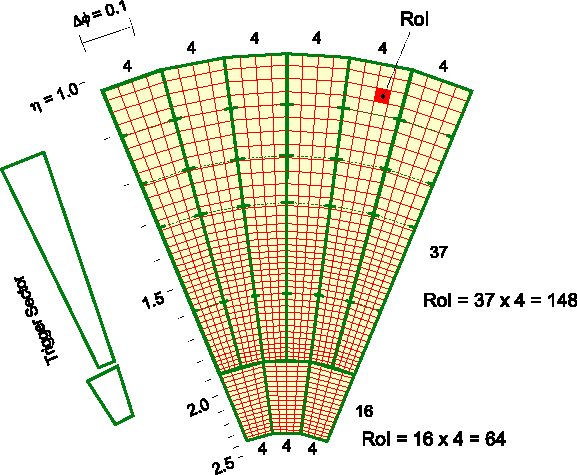
\includegraphics[clip, width=12cm]{fig/3/RoI.pdf}
  \caption{TGCにおけるトリガーセクターとRoIの模式図~\cite{article:phase1}。緑の線で囲まれた領域が1つのトリガーセクターを表し、赤の線で囲まれたマスが1つのRoIを表す。}
  \label{fig:RoI}
\end{figure}



\newpage
\subsection{初段ミューオントリガーにおけるエレクトロニクス}
\ref{section:CW}節で述べたトリガーシステムは様々な電子回路を組み合わせることで実現している。本節では、初段ミューオントリガーで実装されているエレクトロニクスについて述べる。

%初段ミューオントリガーでは、ATLAS 検出器から送られてくる情報に対して SectorLogic、MUCTPI、L1Topo、CTP という電子回路を経てトリガーが発行される。
エンドキャップ部初段ミューオントリガーで用いられるエレクトロニクスは、トリガー判定と検出器のヒット情報の読み出しの2つの役割を担っている。TGCの電子回路とデータの流れを図~\ref{fig:TGC_electro}に示す。
以下では各エレクトロニクスについて説明する。

\begin{figure}[tb]
  \centering
  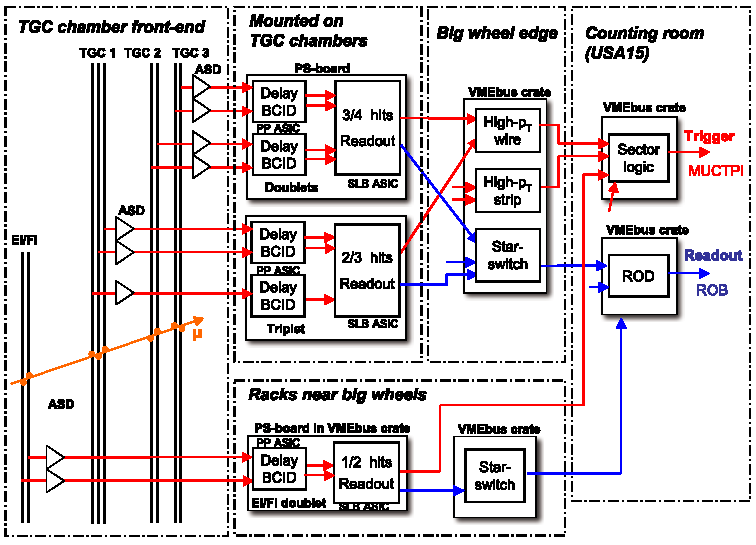
\includegraphics[clip, width=14cm]{fig/3/electronics.pdf}
  \caption{TGC のエレクトロニクスとデータの流れ\cite{Aad:1129811}。赤い線はトリガー信号の流れを、青い線は読み出しデータの流れを示している。}
  \label{fig:TGC_electro}
\end{figure}

\subsubsection{Amplifier Shaper Discriminatorボード}
Amplifier Shaper Discriminator~(ASD) ボードはTGCのワイヤーとストリップからアナログ信号を受け取り、デジタル信号への変換を行う。
ASDボード上のASDにおいてTGCからのアナログ信号を増幅・整形し、閾値電圧を超えた信号のみLVDS信号として出力される。1枚のASDボードは4つのASD-ASICを搭載しており、ASD-ASICは 4 つの信号の受信・処理を行う。そのため、同時に16チャンネルの信号を処理することが可能である。

\subsubsection{Patch-Panel ASIC}
Patch-Panel ASIC~(PP ASIC)はASDからワイヤーとストリップそれぞれのLVDS信号を受け取り、タイミングの調整を行うことで、同じ陽子衝突由来の信号を同時に次のSLB ASICに送る。
陽子衝突が起きてからミューオンが検出器に到達する時間や、ケーブルの長さの違いにより、信号のタイミングが各チャンネルごとに異なるため、PP ASIC を用いてタイミングの調整を行う。

\subsubsection{Slave BoardASIC}
Slave BoardASIC~(SLB ASIC)は読み出しとトリガー判定の 2 種類の処理を行う。
トリガー判定で行う処理としては、各チャンネルの情報を用いてコインシデンスを取ることである。
TGC Triplet~(M1 ステーション)ではワイヤーの3層中2層にヒットがあることを要求し、ストリップの場合は2層中1層にヒットがあることを要求する。
2 つのTGC Doublet~(M2、M3 ステーション)では、各ステーションから信号を受け取りワイヤーとストリップで独立に4層中3層以上にヒットがあることを要求する。これらのコインシデンス結果はLVDS信号で後段のHigh PTボードに送る。

\subsubsection{High PT ボード}
High-PT~(HPT)ボードは、M1のSLBとM2, M3のSLB からのコインシデンス結果を受け取り、M1, M2, M3の3つのステーション間のコインシデンスを行う。M1とM3の位置情報から(d$R$, d$\phi$)を計算し、次のSector Logicに送る。Sector Logicにはボードごとに、位置情報 $R$ と$\phi$、位置の差の情報d$R$とd$\phi$をG-Link通信を用いて送信する。データ通信速度の制限により、1つのHPT-ASICから最大2候補を選んで送信している。

\subsubsection{New Sector Logic}
Sector Logic~(SL)はHPTボードから受け取ったTGC-BWのワイヤー・ストリップの情報と、磁場領域より内側にある検出器から受け取った信号を組み合わせてトリガー判定を行う。
Run-3 では、NSWの導入に伴いトリガー判定に用いるデータ量が増え、従来のSLでは処理できないため刷新された。
まず、TGC-BWのHPTから、ミューオン候補の情報がG-Link通信で送られてくる。この情報からM3のヒット位置のRoIを表す$\eta$、$\phi$及びコインシデンスが取れたM1とのヒット位置のずれ(d$R$, d$\phi$)を取得し、FPGA上に保存されているCoincidence Windowを参照しすることで$p_{\rm{T}}$を判定を行う。
次に、RPC BIS78、Tile カロリメータ、EI/FIからは検出器におけるヒット情報、NSWからは通過したミューオンの飛跡情報が送られてくる。NSWの情報には、ヒット位置を表す$\eta$, $\phi$及びミューオンが飛来した角度$\theta$が含まれる。これらの検出器から送られてくる情報を用いてインナーコインシデンスとりトリガー判定を行う。そして、トリガー判定の結果を後段のMUCTPIに送信する。

\begin{figure}[tb]
  \centering
  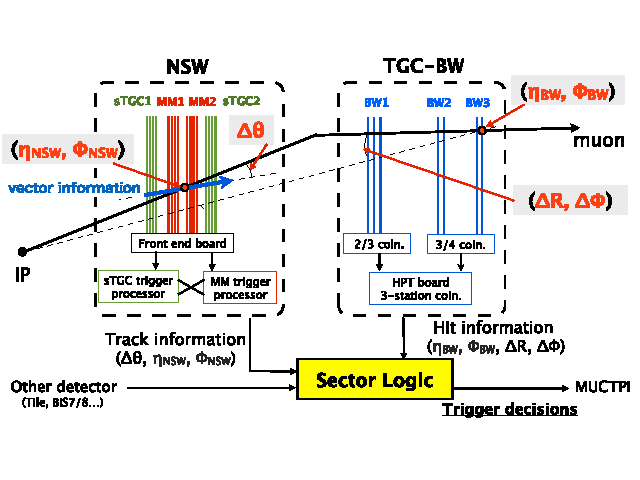
\includegraphics[clip, width=14cm]{fig/2/NSW_innercoin.pdf}
  \caption{Run-3におけるNSWを用いた初段ミューオントリガーの概要図\cite{article:phase1}。NSLにはTGC-BWの他にNSW、RPC BIS78、タイルカロリメータ、EI からの入力がある。これらの検出器からの情報を用いてコインシデンスをとり、トリガー判定を行う。}
  \label{fig:NSW_inner}
\end{figure}


\section{従来のCWの作成及び最適化手法}\label{section:最適化}
\subsection{従来のCWの作成方法}
実際の検出器では磁場構造や構造物による影響などの様々な要素を考慮する必要があるため、CWを数式によって計算し作成するのは困難である。そこで、ミューオンのシミュレーションデータを用いて、ミューオンの$p_{\rm{T}}$と各RoIにおけるd$R$, d$\phi$の対応を調べることでCWを作成している。従来のCWを作成する流れについて以下に述べる~\cite{article:shiomi-mron}。
\begin{enumerate}\label{table:makeCW}
   \item シングルミューオンサンプル(1イベントに対してミューオンが1個のみ存在するシミュレーションサンプル)を用意し、d$R$, d$\phi$の2次元分布図~(ヒットマップ)をRoIごとに作成する。これを、1~GeVから40~GeVまで1~GeV刻みに作成する。
   \item 作成したヒットマップにはミューオンの多重散乱などが原因で、孤立している部分、穴の空いている部分、偶然ヒットした部分が存在する。そこで、ヒットマップのエントリー数などの条件をかけることでヒットマップに対する処理を行う。
   \item 各RoI、各$p_{\rm{T}}$毎に処理を行った40段階の$p_{\rm{T}}$のヒットマップから、15段階のヒットマップを選別する。
   %\item その後、CWの各マスにおける$p_{\rm{T}}$分布をもとに15段階の$p_{\rm{T}}$閾値を選択し、15段階の$p_{\rm{T}}$閾値を持ったCWとしてSLのFPGAに実装する。
   %\caption{隠れ層を構成する要素。}
\end{enumerate}



\subsection{CWの最適化手法}
\subsubsection{TGCの設置位置の測定}\label{ズレ}
TGCは検出器の入れ替えなどのために検出器の移動を行うことがあり、結果として検出器の設置位置(アライメント)にズレが生じてしまう。TGCのアライメントのズレの測定方法はこれまでの研究\cite{article:sano-mron}で既に確立されており、TGCのズレを示すパラメータを図~\ref{fig:dr_para}のように定義する。図~\ref{fig:ズレ}にRun-2での実際のデータを用いて測定したTGCのアライメントのズレの値を示す。TGCの理想位置からの$x$軸方向のズレをd$R$、$z$軸方向のズレを-d$z\tan\theta$と表し、全体としてのズレをd$\rho = dr-dz\tan\theta$と定義する。
d$\rho \textgreater 0$はTGCが動径方向($R$方向)の正の方向にズレていることを表し、d$\rho \textless 0$は負の方向にズレていることを表している。
\begin{figure}[tb]
  \centering
  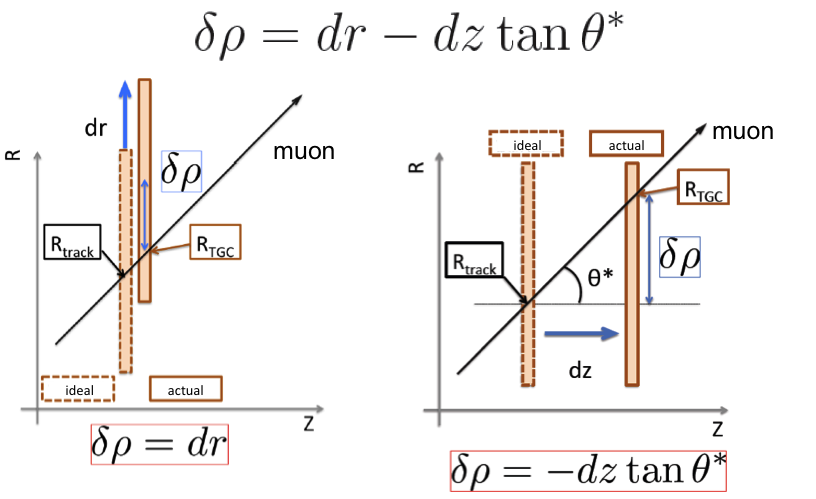
\includegraphics[clip, width=10cm]{fig/3/drho_param_position_measurement.png}
  \caption{TGC 検出器のズレd$\rho$を表すパラメータの定義\cite{article:yamauti-mron}。$x$軸方向のズレをd$R$、$z$軸方向のズレをd$z\tan\theta$と表し、全体としてのズレをd$\rho = $d$r-$d$z\tan\theta$と定義する。}
  \label{fig:dr_para}
\end{figure}

\begin{figure}
    %\begin{tabular}{cc}
    \begin{minipage}[tb]{0.4\linewidth}
        \hspace*{-0.5cm}
        \centering
        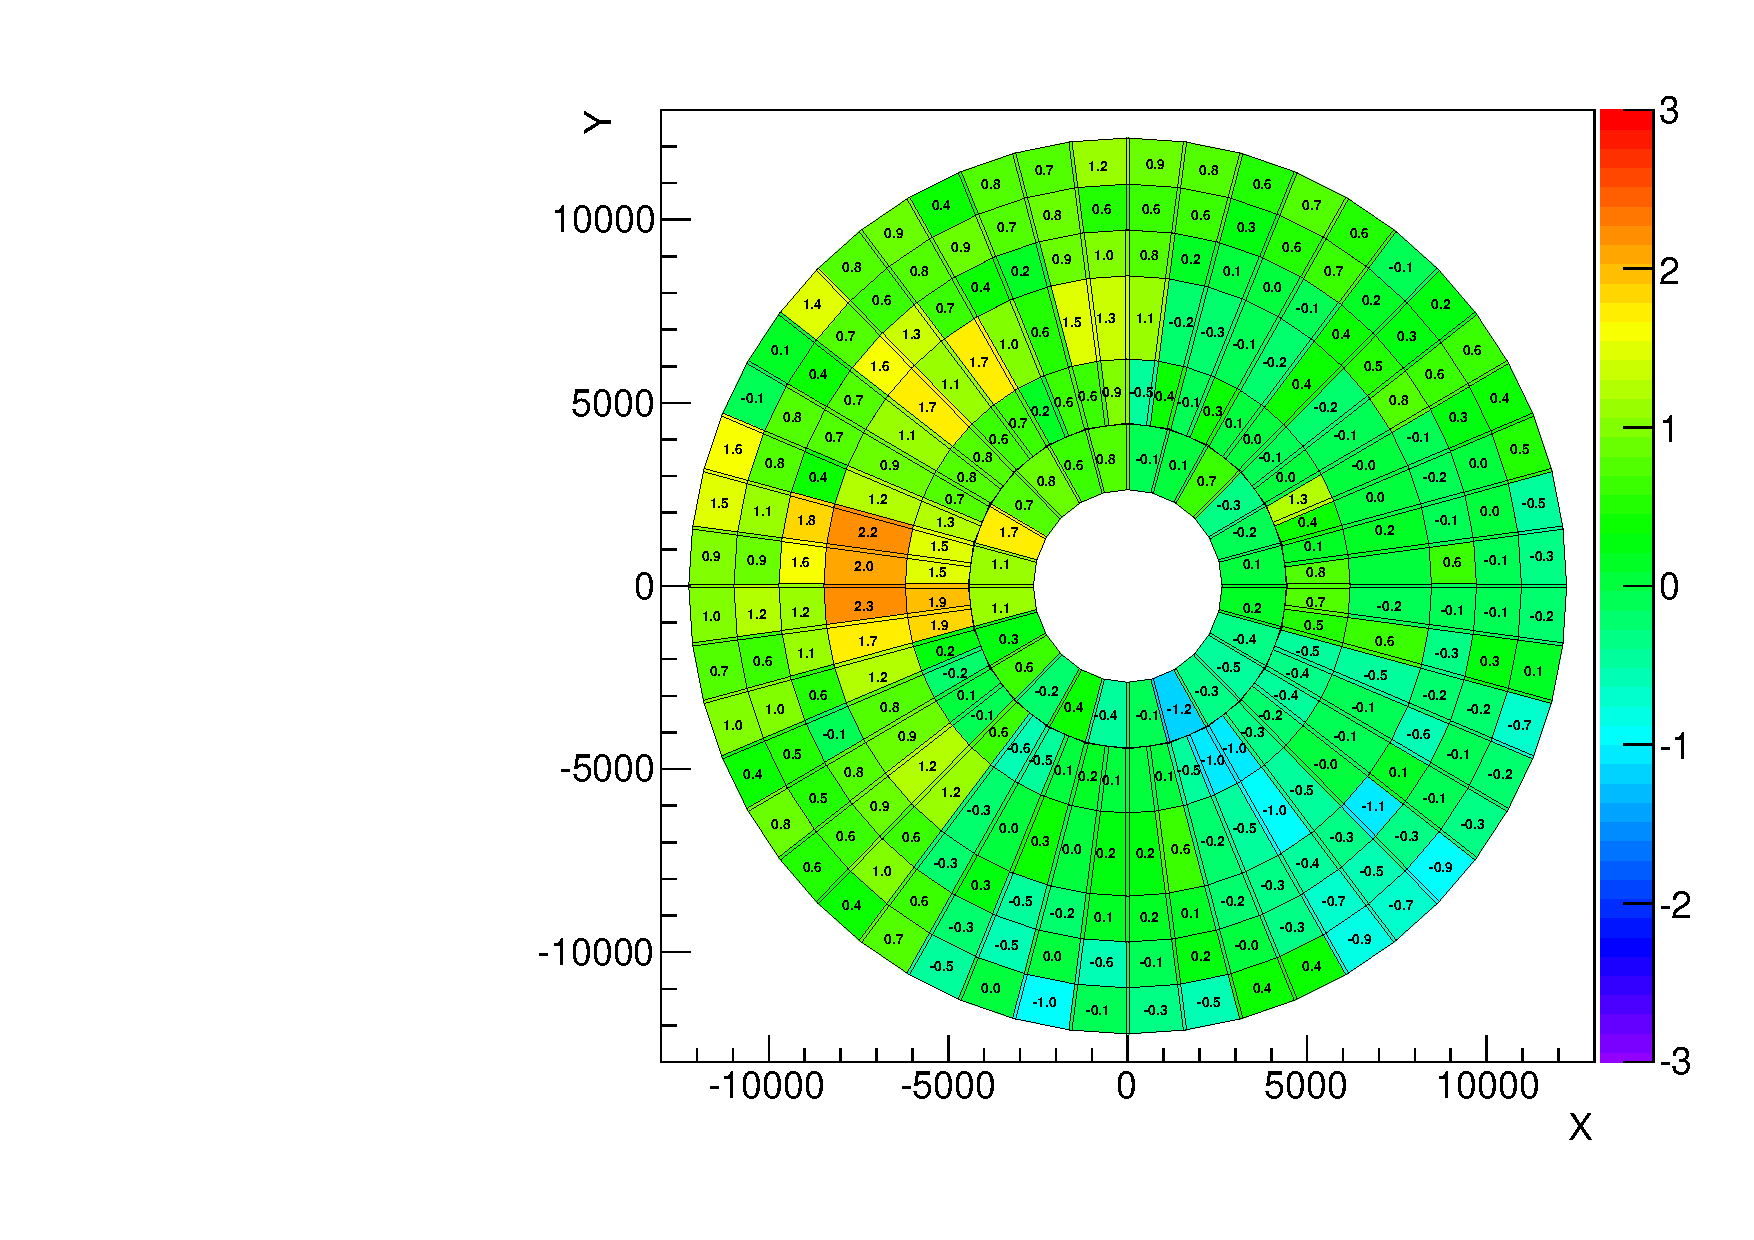
\includegraphics[clip, width=7cm]{fig/3/TGCAlign_CW.muon.bias.20160606.v1.C-side.pdf}
        %\vspace{10pt}
        \subcaption{}
        %\label{}
    \end{minipage}
    \hfill
    \begin{minipage}[tb]{0.4\linewidth}
        \centering
        \hspace*{-1cm}
        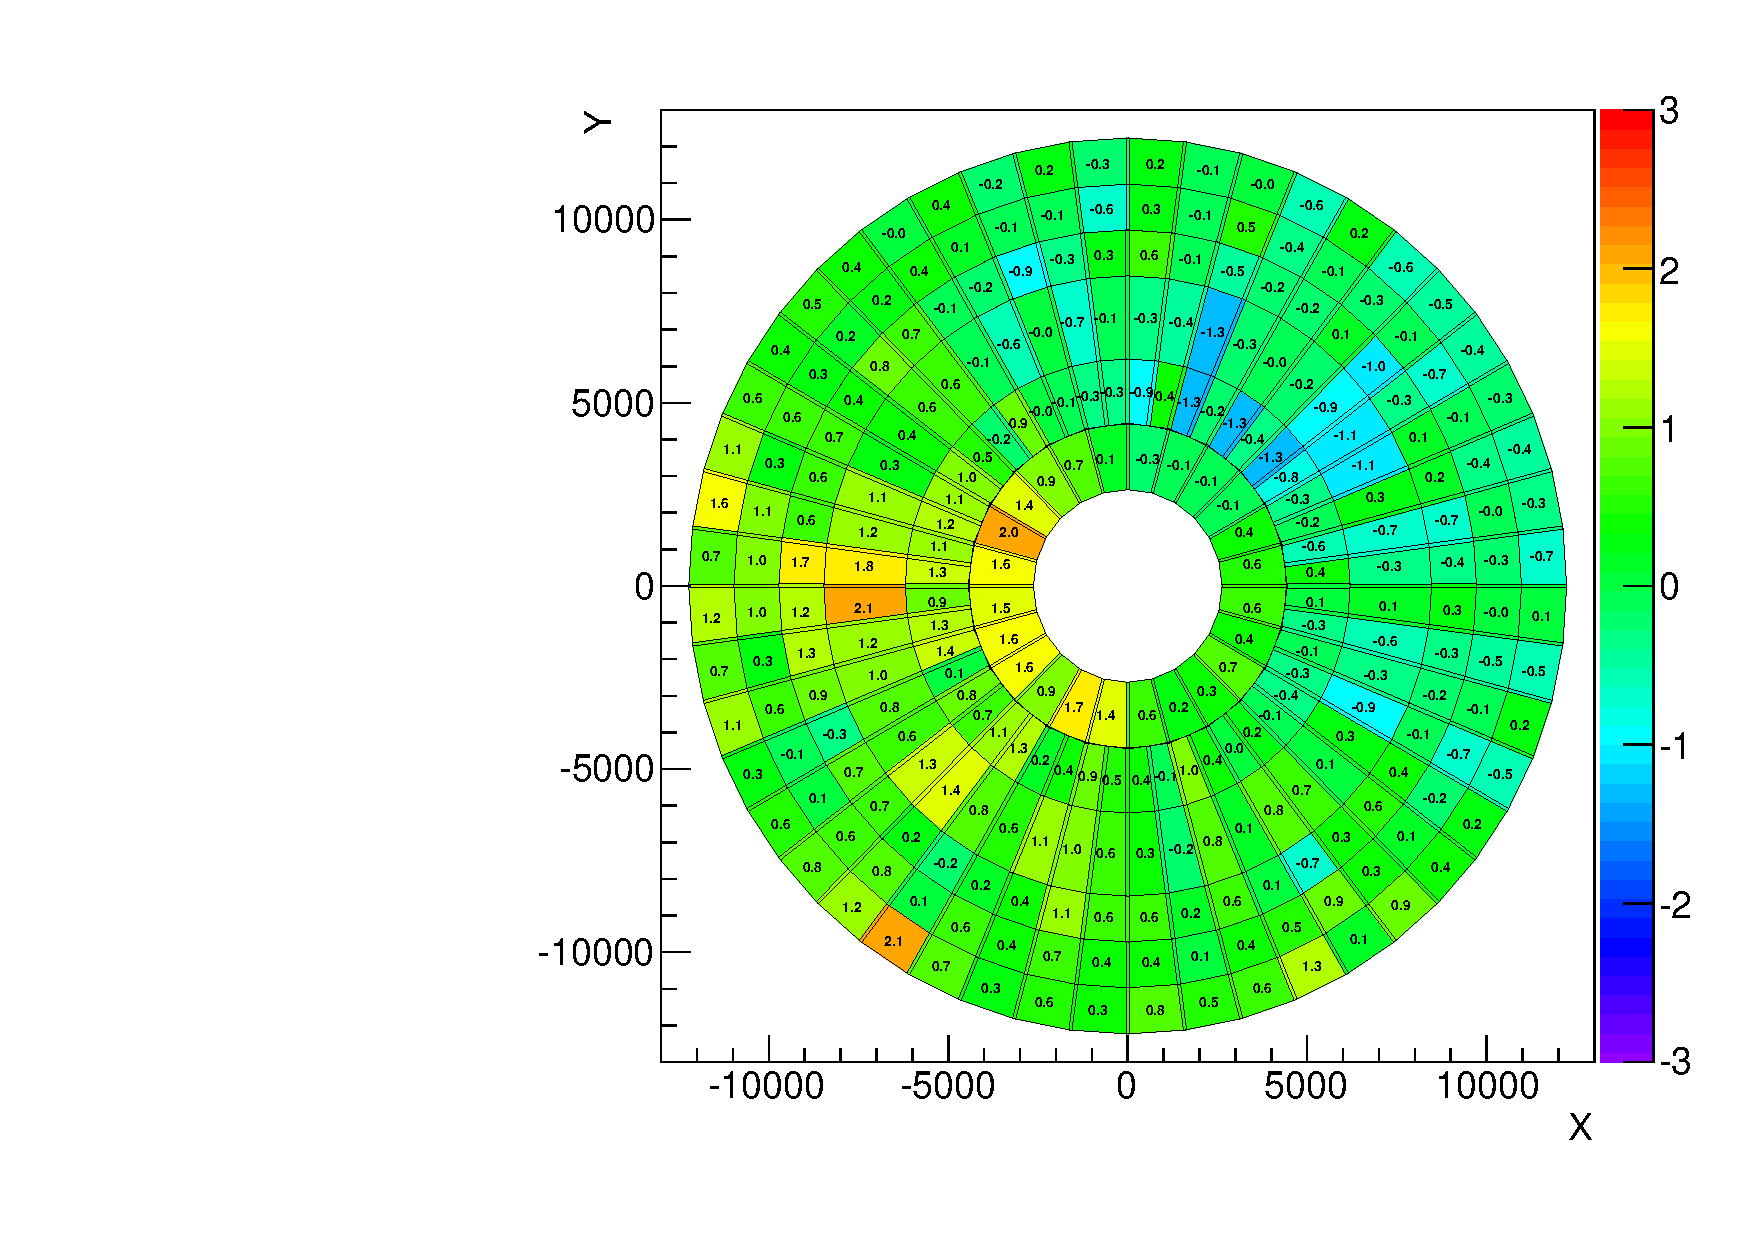
\includegraphics[clip, width=7cm]{fig/3/TGCAlign_CW.muon.bias.20160606.v1.A-side.pdf}
        %\vspace{10pt}
        \subcaption{}
        %\label{}
    \end{minipage}
    \caption{Run-2での検出器のズレの測定図。マスの中の数字がチェンバーごとのズレの値を表す。(a):C-side。(b):A-side。}
    \label{fig:ズレ}
    %\end{tabular}
\end{figure}


\subsubsection{Run-2における最適化手法}
\ref{magnetic_filed}節で述べたように、トロイド磁石によって8回転対象の磁場構造が形成されている。そのため、従来の手法ではシミュレーションデータを用いて1回転分のCWを作成し、1つのCWをTGC-BWの8か所に対応させていた。
しかし、シミュレーションにおいてTGCは設計通りの位置に設置されているが、実際の検出器ではアライメントにズレが生じている。
このため、検出器アライメントのズレのせいで、TGCにおける磁場構造は厳密には8回転対象ではなくなっている。しかし、シミュレーションをもとに、8回転対象を前提としたCWには実際の検出器アライメントのズレの影響が考慮されていない。そのため、このCWをトリガーに適応するとミューオントリガーの運動量分解能の低下やトリガーレートの増加を招く原因となる。
そこで、トリガー性能の向上のためにはCWに補正を行い検出器アライメントに対して最適化する必要がある。

Run-2におけるCWの最適化方法は先行研究で開発されており、$p_{\rm{T}}$が11~GeV, 15~GeV, 20~GeVの閾値に対して最適化を行ったことでトリガー性能が改善された\cite{article:kido-mron}。
ここで行われていた手法では、実際のデータから検出器のズレの大きさを各TGCチェンバー毎に見積もり、その値に従ってCWに補正を加えることでトリガー効率を改善させていた。
%そこで、Run-2では実際のデータからTGCのズレの大きさを各チェンバー毎に見積もり、その値に従ってCWに補正を加えることでトリガー効率を改善させていた。
%シミュレーションにおいてTGCは設計通りの位置に設置されているが、実際の検出器では設置位置(アライメント)にズレが生じている。
%従来のCWの作成手法では、シミュレーションデータを使用し作成するため、CWには実際のTGCの設置位置によるズレの影響が考慮されていない。そのため、このCWをトリガーに適応するとミューオントリガーの運動量分解能の低下やトリガーレートの増加を招く原因となる。
%CWの補正方法は先行研究で確立されており、Run-2ではL1 MU15及L1 MU20の2つの閾値にのみ補正を行った結果、トリガー性能が改善された\cite{article:kido-mron}。
以下にシミュレーションデータから作成されたCWにおける$p_{\rm{T}}$閾値が20~GeVのトリガーに対するRun-2で行われた最適化の流れを示す。
\begin{enumerate}\label{table:CW_optimazation}
   \item Run-2 の実データから$p_{\rm{T}}<20$GeVのd$R$, d$\phi$の情報を抜き出し、d$R$, d$\phi$のヒットマップを各RoI毎に作成する。
   \item 作成したヒットマップに対して、ヒットマップの各マスごとに式~\eqref{equ:Aliment}で定義するパラメータxを計算する。
   \begin{equation}
        x = \frac{N_{p_{\rm{T}} > 20~\rm{GeV}}}{\sqrt{N^2_{p_{\rm{T}} > 20~\rm{GeV}}+N^2_{p_{\rm{T}} < 20~\rm{GeV}}}}
       \label{equ:Aliment}
   \end{equation}
   ここで、$N_{p_{\rm{T}} > 20~\rm{GeV}}$はヒットマップのマスにおける$p_{\rm{T}} > 20$~GeVのミューオン数、$N_{p_{\rm{T}} < 20~\rm{GeV}}$はヒットマップのマスにおけるのミューオン数である。
   \item すべてのヒットマップの各マスでで計算した$x$の値を指針として、CWのマスが示す$p_{\rm{T}}$閾値が正しいかどうかを判断し、必要に応じてCWの閾値を一段階変更する。
   %\caption{隠れ層を構成する要素。}
\end{enumerate}
この手順を各$p_{\rm{T}}$閾値に対して上の閾値から順番に行うことでCWの最適化を行う。

\section{本研究の目的}
2022年の運転で一時的に瞬間ルミノシティ$2.5\times10^{34}~{\rm cm^{-2}s^{-1}}$まで到達したことを受け、2023年以降の運転ではより高いルミノシティで安定した運転を行うことが予定されている。そのため、2022年度の初段ミューオントリガーのままではトリガーレートが大幅に増加してしまうため、さらなるトリガー性能の向上が喫緊の課題である。

トリガーシステムの改善にはいくつか方法があるが、その中でもCWに対して検出器アライメントの補正を行う方法がある。
ATLAS検出器のトロイド磁石は等間隔に8個設置されており、8回転対象の磁場構造が形成されている。そのため、従来の手法ではシミュレーションデータを用いて1回転分のCWを作成することで、8回転のすべての箇所に適応することができた。
しかし、実際には検出器アライメントのズレによって、TGCにおける磁場構造は厳密には8回転対象ではなくなってしまい、トリガー性能の向上のためにはRoIごとにCWに対して補正を行い最適化する必要がある。


Run-2では\ref{section:最適化}節で示すように、先行研究によって開発された手法を用いて手動で補正を行っていたが、この手法は$p_{\rm{T}}$閾値に対して柔軟な対応が難しい上に補正には多大な作業量が必要になってくる。そのため、15段階に増設されたRun-3の$p_{\rm{T}}$閾値に対して従来の手法で補正を行うことが難しい。そこで、従来の手法に代わってRun-3の15段階閾値に対応したCWを効率よく補正する手法の開発が必要である。

本研究では効率化する方法として、近年急速に発展している機械学習に着目し、機械学習を用いた新たなCWの最適化手法の開発を行う。
機械学習は近年大きな注目を集めている技術あり、様々な分野で活用されている。機械学習とは、人がコンピュータにルールや知識を明示的に与える代わりに、学習するためのデータを与え、コンピュータ自身がそのデータからルールや知識を獲得する手法である。そのため、ATLAS実験で実際に取得したデータを機械学習に与えることで、多大な作業量を必要とするCWの作成及び最適化の作業に対して効率化が期待できる。
%\ref{section:最適化}節で示すように、従来の手法ではシミュレーションデータからCWを作成し、実際のデータのを用いて検出器のズレに対する補正を手動で行っていた。
%ATLAS実験では、初段ミューオントリガーのアップグレードに伴ってRun-3に対応したCWを作り直す必要があり、Run-3においてもトリガー性能を向上させるためにはCWの最適化を行う必要がある。しかし、Run-2で行われていた最適化手法は膨大な作業量であり2つの$p_{\rm{T}}$閾値のみにしか最適化を行うことができなかった。そのため、$p_{\rm{T}}$閾値が15段階あるRun-3のCWに対して、Run-2と同様の作成及び最適化手法を行うことは現実的でない。
%そこで、従来の手法に代わってRun-3に対応したCWを効率よく作成し最適化する手法の開発が必要である。
%そこで、本研究では効率化する方法として、近年急速に発展している機械学習に着目した新たなCWの作成及び最適化手法の開発を行う。
%機械学習は近年大きな注目を集めている技術あり、様々な分野で活用されている。機械学習とは、人がコンピュータにルールや知識を明示的に与える代わりに、学習するためのデータを与え、コンピュータ自死因がそのデータからルールや知識を獲得する手法である。「複数人の専門家が数年かかって作っていく」ようなルールや知識などは、作成自体にも、作成後の調整や変更にも膨大な時間とコストがかかるが、機械学習を用いることで学習用のデータを機械にかけて数日待てば自動的に作成することができるのである。そのため、多大な作業量を必要とするCWの作成及び最適化の作業に対しても、機械学習を用いることで効率化が期待できる。




%また、ミューオンの電荷にも影響がある。
%\begin{figure}[tb]
%  \centering
%  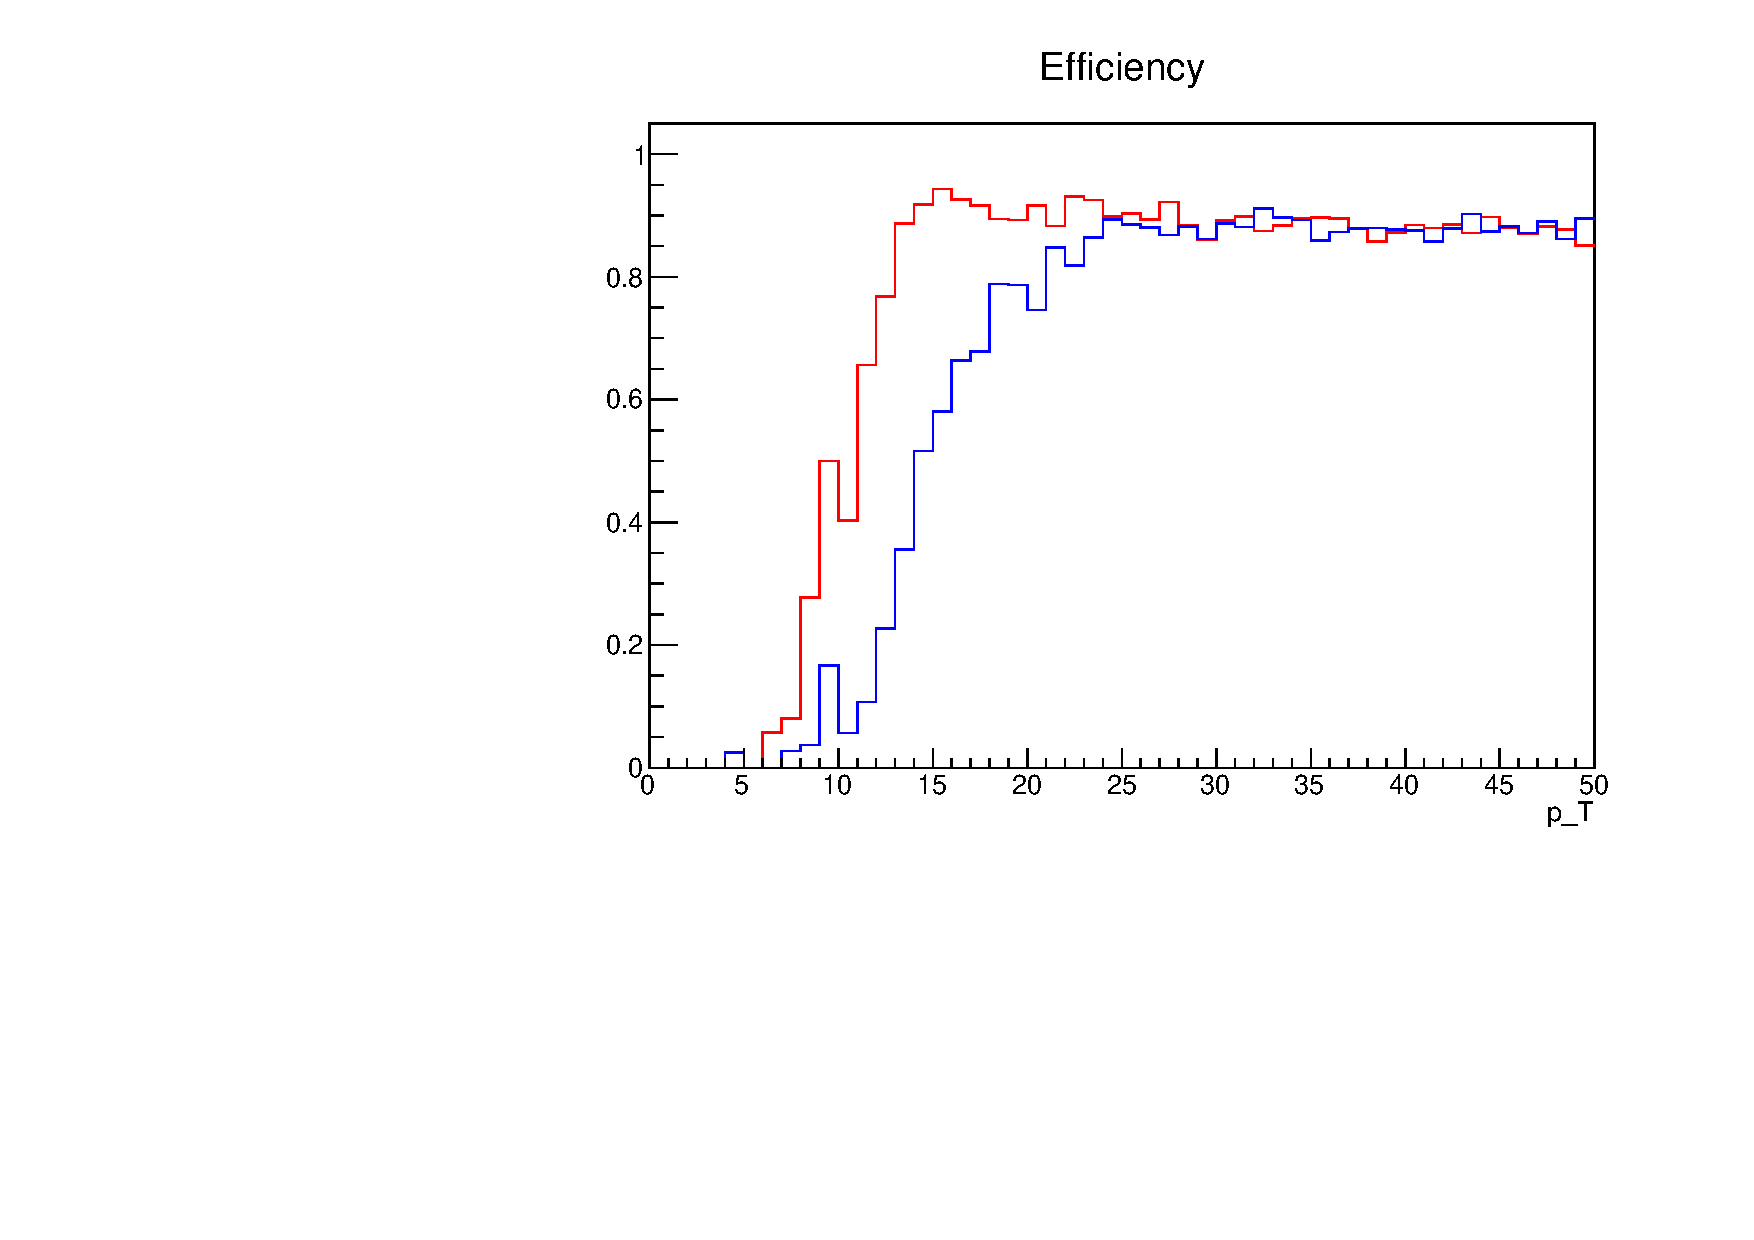
\includegraphics[clip, width=7cm]{fig/3/charge_14gev_phi2_eta11.pdf}
%  \caption{あるチェンバーにおける電荷別のTurn-on curveの例。赤が正電荷、青が負電荷のTurn-on curveである。}
%  \label{fig:fit_def}
%\end{figure}









